\chapter{Przebieg badań}
Doświadczenie polegało na analizie porównawczej sprawności algorytmów opisanych w \refsource{rozdziale}{cha:dos} w \refsource{sekcji}{sec:alg}. Celem doświadczenia było określenie jakości algorytmu utworzonego w ramach pracy inżynierskiej autora\cite{Blyszcz2022}. Szczegółowa metodologia badawcza została określona w \refsource{podrozdziale}{sec:met}.

\section{Metodologia badawcza}
\label{sec:met}
Przyjęta w projekcie metodologia badawcza została określona w poniższej \refsource{tabeli}{tab:met-bad}. Przyjęta metodologia ma za zadanie określić jakoś porównywanego algorytmu.

\begin{table}[H]
    \centering
    \captionsource{Metodologia badawcza}{Opracowanie własne}
    \begin{tabular}{|L{\textwidth}|}
        \hline
        \textbf{Problem badawczy:} \\
        Czy algorytm klasyfikacji danych utworzony w ramach pracy inżynierskiej może konkurować z rozwiązaniami dostępnymi w środowiskach komercyjnych \\ \hline

        \textbf{Pytania badawcze:} \\
        \begin{enumerate}
            \item Czy algorytm jest konkurencyjny pod względem wybranych metry:
            \begin{itemize}
                \item dokładność algorytmu
                \item czas działania
                \item precyzja
                \item czułość
                \item f1
                \item auc
            \end{itemize}
        \end{enumerate} \\ \hline

        \textbf{Hipotezy:} \\
        \begin{enumerate}
            \item Nie ma istotnej różnicy w uzyskanej ''\textit{dokładności}'' między algorytmami.
            \item Nie ma istotnej różnicy w uzyskanej ''\textit{czułości}'' między algorytmami.
            \item Nie ma istotnej różnicy w uzyskanej ''\textit{precyzji}'' między algorytmami.
            \item Nie ma istotnej różnicy w uzyskanym ''\textit{auc}'' między algorytmami.
            \item Nie ma istotnej różnicy w uzyskanej ''\textit{f1}'' między algorytmami.
            \item Nie ma istotnej różnicy w uzyskanym ''\textit{czasie działania}'' między algorytmami.
        \end{enumerate} \\ \hline
    \end{tabular}
    \label{tab:met-bad}
\end{table}

\section{Przygotowanie platformy}
Do badań wykorzystano narzędzie ''\textit{Projektant}'' znajdujące się na platformie ''\textit{Azure Machine Learning Studio}'' (Azure ML). Narzędzie to umożliwiło utworzenie interaktywnego potoku zadań. Potok ten składa się z kilku części:
\begin{itemize}
    \item Przygotowanie i obróbka zbiorów danych
    \item Trenowanie oraz testowanie algorytmów klasyfikacji danych
    \item Utworzenie tabeli porównawczej dla wyników poszczególnych algorytmów (\refsource{obraz}{fig:pipeline}).
\end{itemize}

\subsection{Przygotowanie danych}
W pierwszym kroku dane zostały znormalizowane za pomocą metody \textbf{MinMax}, która przekształca dane numeryczne do wartości w zakresie ${0, 1}$. W następnym kroku za pomocą języka Python oraz biblioteką Pandas oraz Numpy zostają zamienione etykiety słowne na wartości \textbf{0} i \textbf{1} oraz następuje zamiana wartości $[NaN, -inf, inf]$ na cyfrę $0$. Cały proces został zobrazowany na \refsource{diagramie}{fig:norm}

\begin{figure}[H]
    \centering
    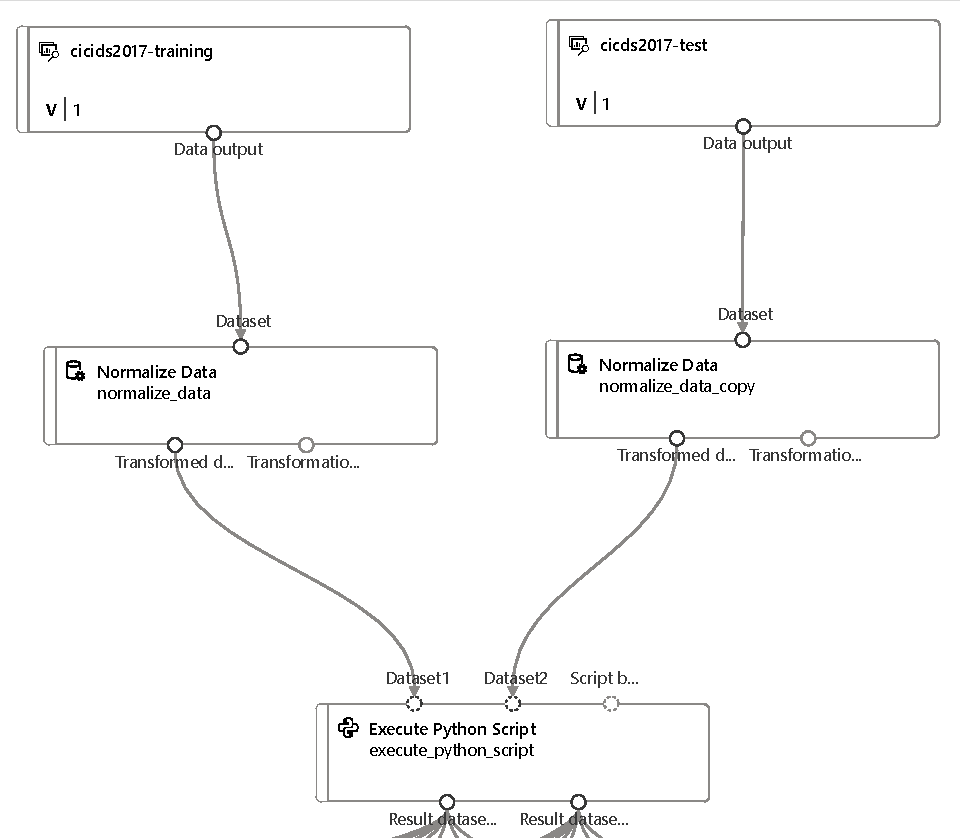
\includegraphics[width=0.6\textwidth]{images/norm}
    \captionsource{Potok normalizacji danych}{Opracowanie własne}
    \label{fig:norm}
\end{figure}

\subsection{Trenowanie oraz testowanie algorytmów}
Kolejną grupą zadań widoczną w potoku są te związane z trenowaniem i testowaniem poszczególnych algorytmów opisanych w \refsource{rozdziale}{cha:dos}. Każdy test składa się 3 kafelek. W przypadku algorytmów dostarczonych wraz z platformą Azure ML są to:
\begin{itemize}
    \item \textbf{model klasyfikujący} - odpowiada za przygotowanie algorytmu klasyfikacyjnego
    \item \textbf{blok treningowy} - tworzy wytrenowany model, za pomocą połączonego zbioru danych
    \item \textbf{blok ewaluacyjny} - sprawdza wcześniej wytrenowany model za pomocą powiązanego zbioru danych.
\end{itemize}
Potok zadań wykorzystujący algorytmy dostarczone przez Microsoft Azure został ukazany na \refsource{schemacie}{fig:ms-pipe}

\begin{figure}[H]
    \centering
    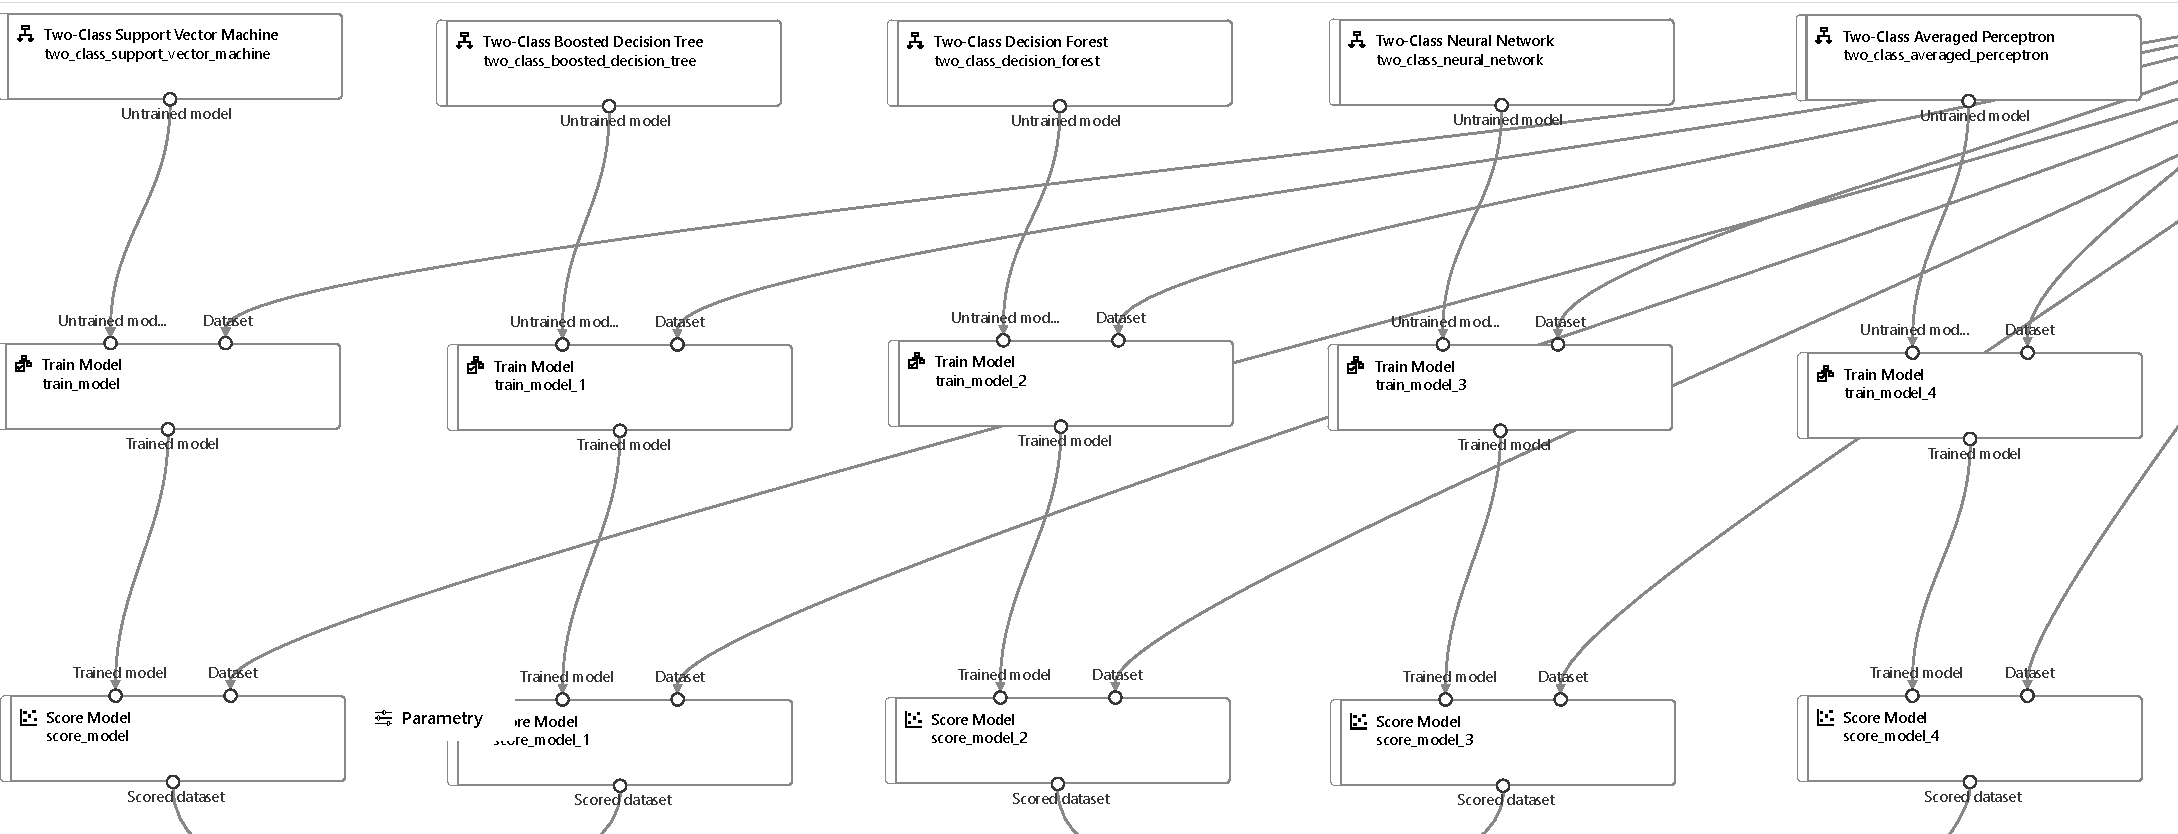
\includegraphics[width=\textwidth]{images/ms_pipe}
    \captionsource{Potok zadań dla algorytmów klasyfikacyjnych}{Opracowanie własne}
    \label{fig:ms-pipe}
\end{figure}

Algorytmy dostarczone w ramach pracy badawczej składają się z:
\begin{itemize}
    \item \textbf{biblioteka Python} - archiwum o rozszerzeniu \textbf{.zip}, które zawiera w sobie odpowiednie pliki napisane w języku Python
    \item \textbf{blok treningowy} - wykorzystuje dostarczoną bibliotekę do wytrenowania modelu oraz zapisania na platformie Azure najlepszego uzyskanego wyniku za pomocą powiązanego zbioru danych
    \item \textbf{blok ewaluacyjny} - wykorzystuje dostarczoną bibliotekę do ewaluacji algorytmu za pomocą połączonego zbioru danych
\end{itemize}

Potok zadań dla algorytmów niestandardowych został ukazany na \refsource{rysunku}{fig:au-pipe}

\begin{figure}[H]
    \centering
    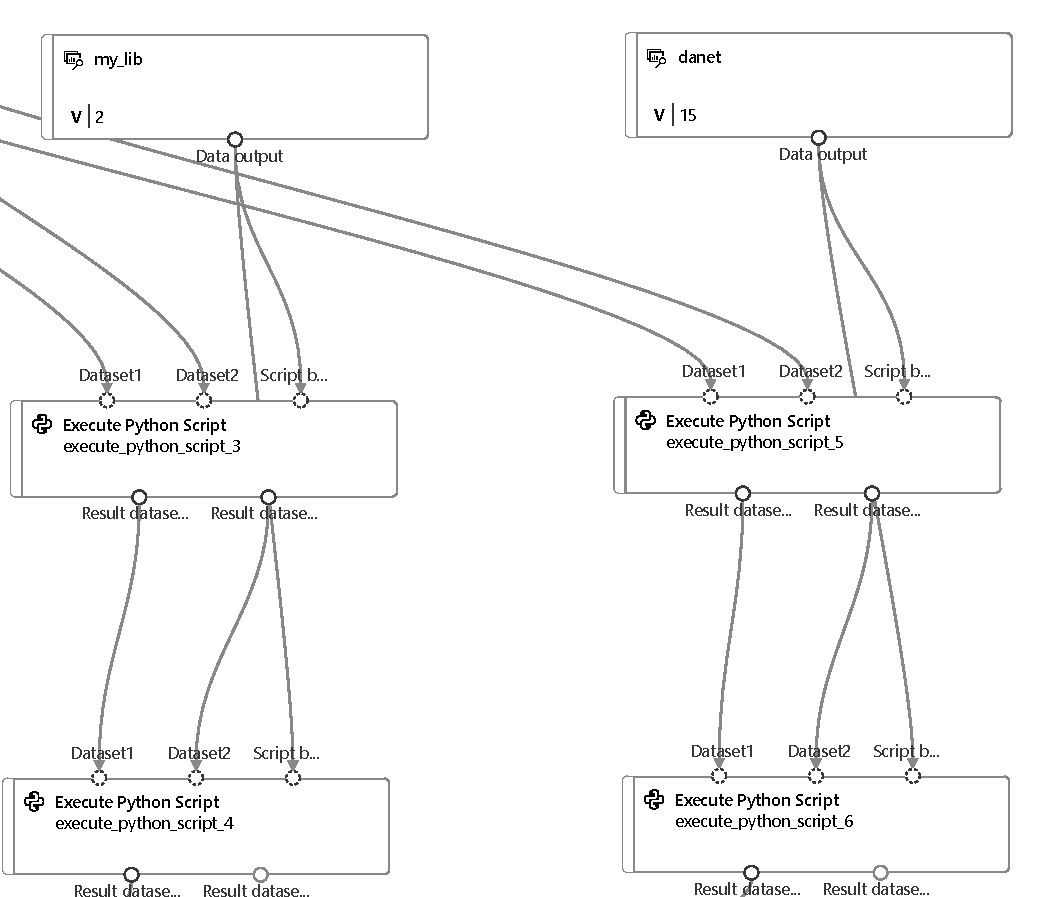
\includegraphics[width=0.8\textwidth]{images/au-pipe}
    \captionsource{Potok zadań dla algorytmów klasyfikacyjnych}{Opracowanie własne}
    \label{fig:au-pipe}
\end{figure}


\subsection{Utworzenie tabeli porównawczej}
Kolejną częścią zadań jest zebranie wyników poszczególnych algorytmów oraz połączenie ich w jedną całość. Wykorzystano do tego moduły języka Pyton, które zwracają przetwożone wyniki oraz łączą je w jedną tabelę zbiorczą, co pokazano na \refsource{rysunku}{fig:pipe-4}.

\begin{figure}[H]
    \centering
    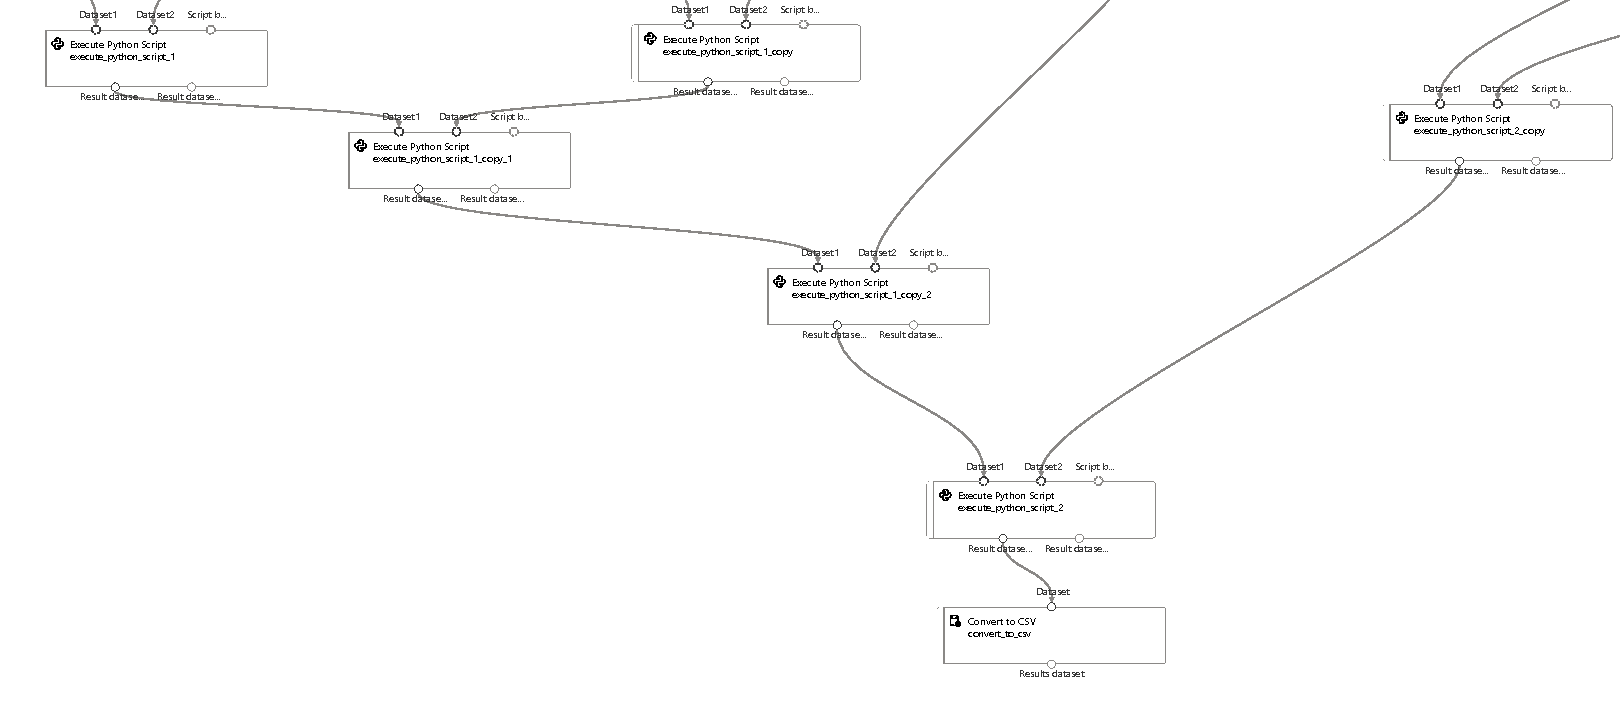
\includegraphics[width=\textwidth]{images/pipe-csv}
    \captionsource{Moduły odpowiedzialne za przetwożenie wyników}{Opracowanie własne}
    \label{fig:pipe-4}
\end{figure}

\section{Weryfikacja potoku}
Aby zweryfikować działanie całego procesu wykorzystano znormalizowane dane treningowe do wytrenowania oraz przetestowania działania algorytmów klasyfikacyjnych. Cały proces trwał ''\textbf{1 dzień 10 godzin 55 minut 53 sekundy}''. Wyniki tych działań widać na \refsource{rysunku}{fig:predict-same}. Analizując wykres można zauważyć, że uzyskane wyniki znajdują się w przedziale $[94\%, 100\%]$ w każdej metryce co pokazuje jakość każdego z algorytmów, a także to, że algorytmy poradziły sobie niemal bezbłędnie w rozpoznawaniu ruchu sieciowego, na którym były uczone. Zbiór, który wykorzystano do trenowania oraz testowania danych zawierał w sobie 225805 wpisów z czego 97718 należało do klasy ''\textbf{1}'', zaś 128087 należało do klasy ''\textbf{0}''.

\begin{table}[H]
    \centering
    \captionsource{Liczba elementów przynależących do danej klasy w zniorze treningowym}{Opracowanie własne}
    \label{tab:trening-data-label}
    \begin{tabular}{|c|r|} \hline
        \textbf{Klasa} & \textbf{Liczba wystąpień} \\ \hline
        1 & 97718 \\ \hline
        0 & 128027 \\ \hline
        \textbf{Suma} & 225805 \\ \hline
    \end{tabular}
\end{table}

Bazując na tym zbiorze oraz uzyskanych wynikach udało się udowodnić poprawność działania procesu klasyfikacji wieloma algorytmami genetycznymi.

\begin{landscape}
    \vspace*{\fill}
    \begin{figure}[H]
        \centering
        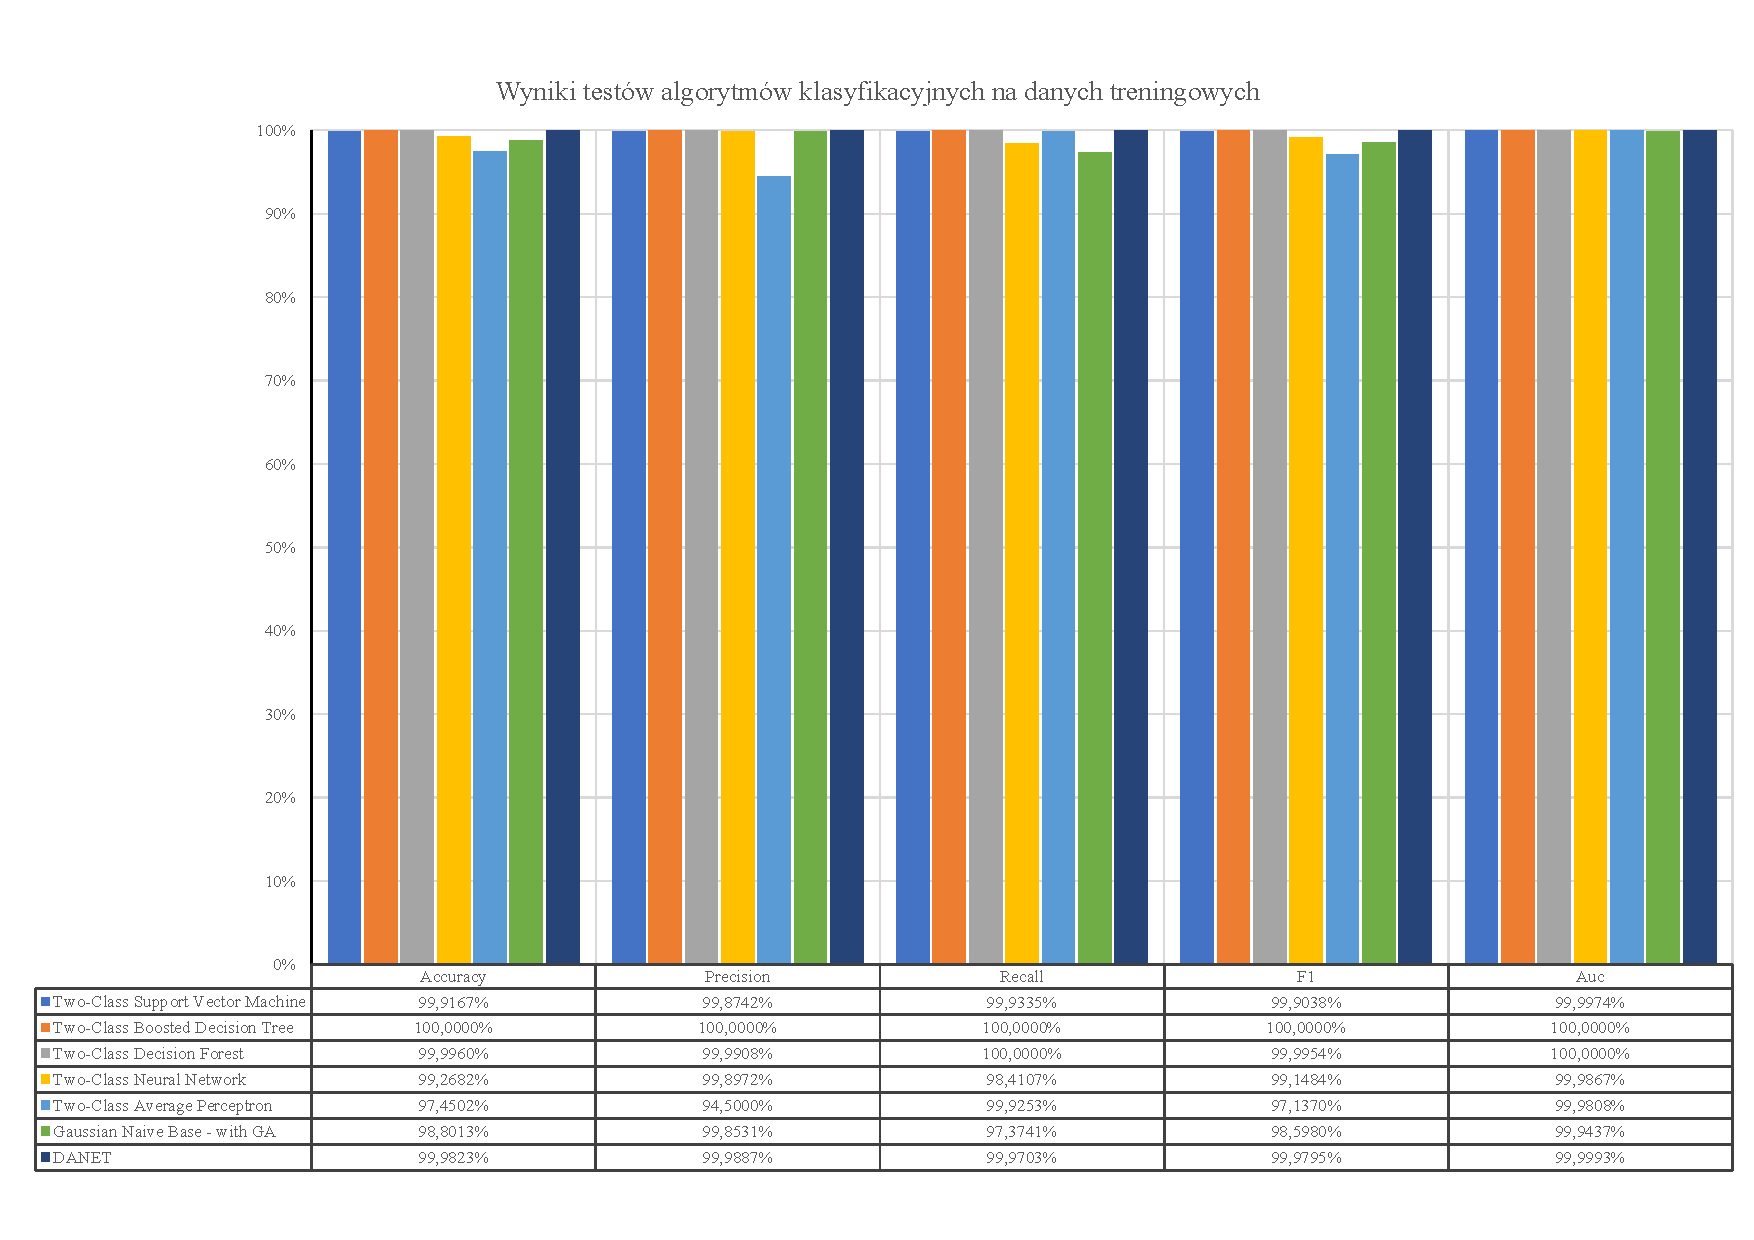
\includegraphics[height=0.8\textwidth]{images/predict_same}
        \captionsource{Wyniki testów algorytmów klasyfikacyjnych na danych treningowych}{Opracowanie własne}
        \label{fig:predict-same}
    \end{figure}
\vfill

\end{landscape}

\section{Próba badawcza}
Aby uzyskać realne wyniki podczas porównywania poszczególnych algorytmów zastosowano zbiór treningowy opisany w \refsource{tabeli}{tab:trening-data-label} oraz zbiór testowy, który zawierał 2273097 wpisów należących do klasy ''\textbf{1}'' oraz 557646 wpisów należących do klasy ''\textbf{0}'' co sumarycznie daje: 2830743 wpisów tak jak to zostało pokazane w \refsource{tabel}{tab:res-test}.

\begin{table}[H]
    \centering
    \captionsource{Liczba elementów przynależących do danej klasy w zbiorze testowym}{Opracowanie własne}
    \label{tab:res-test}
    \begin{tabular}{|c|r|} \hline
        \textbf{Klasa} & \textbf{Liczba wystąpień} \\ \hline
        1 & 2273097 \\ \hline
        0 & 557646 \\ \hline
        \textbf{Suma} & 2830743 \\ \hline
    \end{tabular}
\end{table}

Podczas analizy można zauważyć fakt, że algorytm DANet odstaje od pozostałych algorytmów w rezultatach mierzonych większością metryk. Dokładność na poziomie $19,9691\%$ pokazuje fakt, że algorytm poprawnie zaklasyfikował jedynie $565273$ wpisów. Wynik taki pokazuje, że ten algorytm jest niewystarczający do tego problemu dlatego został wykluczony z dalszych porównań.

\subsection{Dopasowanie}
Wśród pozostałych algorytmów najlepsze dopasowanie uzyskał algorytm: ''\textit{Two-Class Average Perceptron}'', którzy uzyskał wynik na poziomie $85,776\%$, zaś najgorzej poradził sobie ''\textit{Two-Class Support Vector Machine}'' uzyskując $80,3002\%$ w teście. Mimo tego te 6 algorytmó uzyskało podobne wyniki mieszczące się w granicy 3 punktów procentowych różnicy od średniego dopasowania. Algorytm autora (''\textit{Gaussian Naive Base - with GA}'') (GAGNB) uzyskał w tym teście $80,3004\%$. Wyniki zostały przedstawione w \refsource{tabeli}{tab:acc-res} oraz na \refsource{wykresie}{fig:acc-res}.

\begin{table}[H]
    \centering
    \captionsource{Wynik dopasowania algorytmów}{Opracowanie własne}
    \begin{tabular}{|l|r|} \hline
        \textbf{Algorytm} & \textbf{Wartość} \\ \hline
        Two-Class Support Vector Machine & $80,3002\%$ \\ \hline
        Two-Class Boosted Decision Tree & $83,8482\%$ \\ \hline
        Two-Class Decision Forest & $83,1725\%$ \\ \hline
        Two-Class Neural Network & $84,7332\%$ \\ \hline
        Two-Class Average Perceptron & $85,7768\%$ \\ \hline
        Gaussian Naive Base - with GA & $80,3004\%$ \\ \hline
        \end{tabular}
    \label{tab:acc-res}
\end{table}

\begin{landscape}
    \vspace*{\fill}
    \begin{figure}[H]
        \centering
        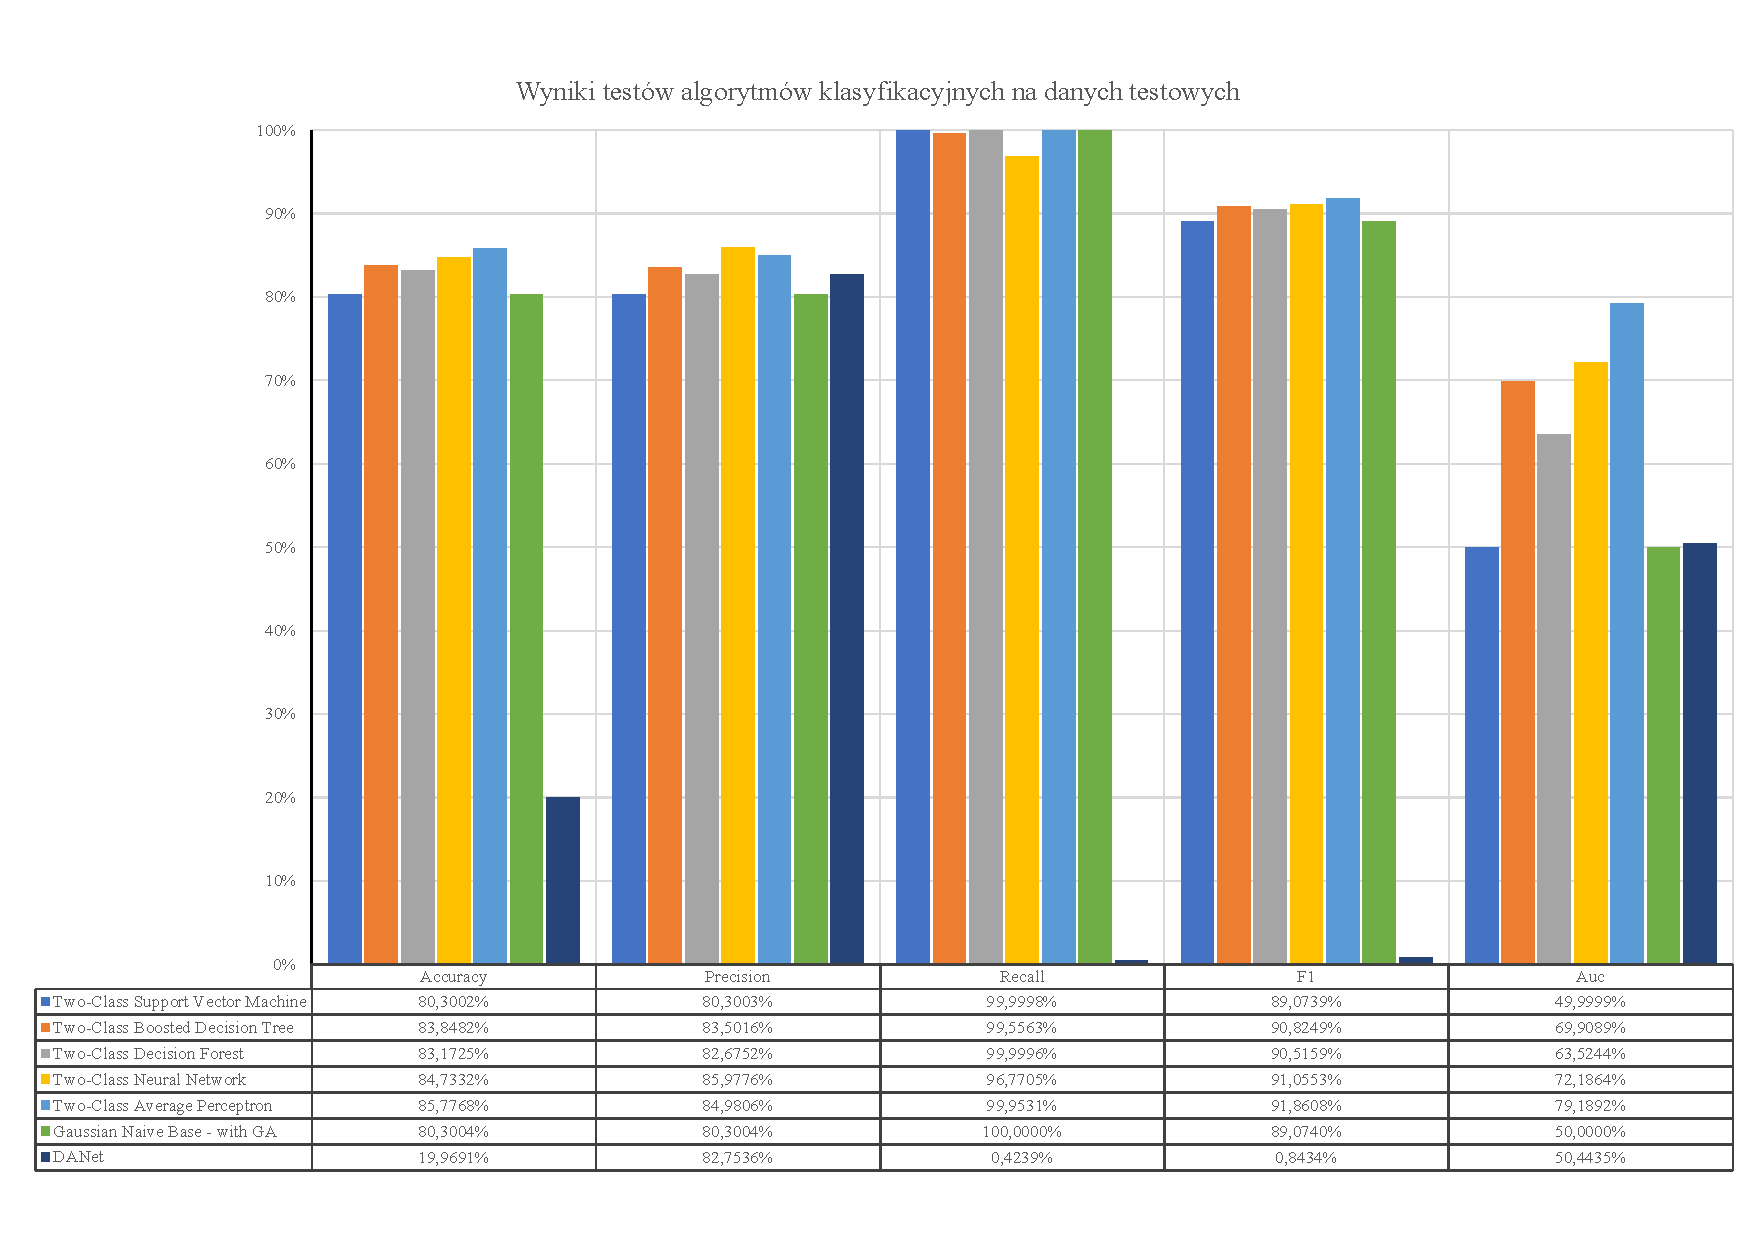
\includegraphics[height=0.8\textwidth]{images/predict_result}
        \captionsource{Wyniki testów algorytmów klasyfikacyjnych na danych testowych}{Opracowanie własne}
        \label{fig:predict-result}
    \end{figure}
    \vfill
\end{landscape}


\begin{figure}[H]
    \centering
    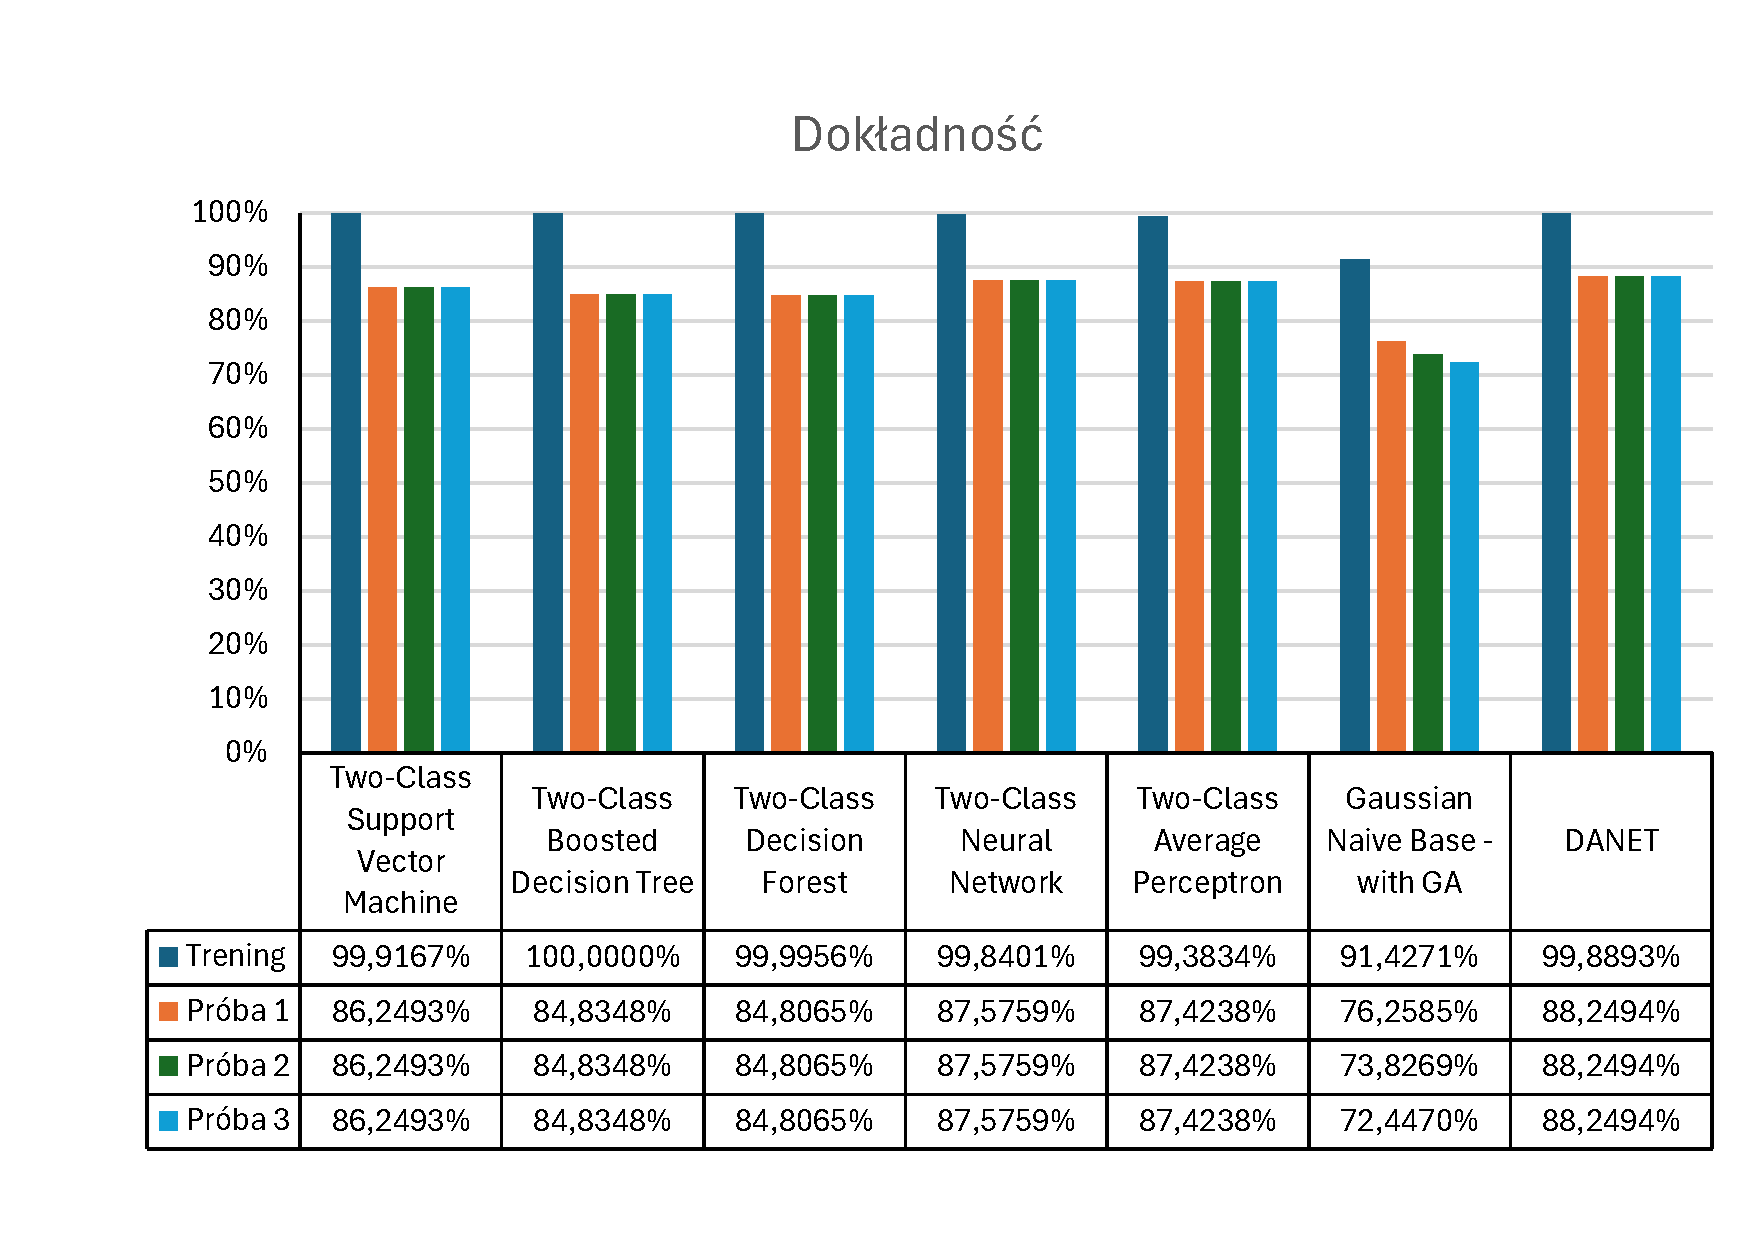
\includegraphics[width=\textwidth]{images/acc-res}
    \captionsource{Dokładność algorytmów}{Opracowanie własne}
    \label{fig:acc-res}
\end{figure}

\subsection{Precyzja}
Najlepszy wynik precyzji uzyskał algorytm ''\textit{Two-Class Neural Network}'' ($85,9776\%$) co oznacza, że najlepiej poradził sobie z dopasowaniem ruchu klasy ''\textbf{1}''. Najsłabszy wynik uzyskał ''\textit{Two-Class Support Vector Machine}'' ($80,3003\%$). GAGNB uzyskał $80,3004\%$ precyzji. Wyniki są opisane w \refsource{tabeli}{tab:acc-prec} oraz na \refsource{wykresie}{fig:acc-prec}.

\begin{table}[H]
    \centering
    \captionsource{Wynik precyzji algorytmów}{Opracowanie własne}
    \begin{tabular}{|l|r|} \hline
    \textbf{Algorytm} & \textbf{Wartość} \\ \hline
    Two-Class Support Vector Machine & $80,3003\%$ \\ \hline
    Two-Class Boosted Decision Tree & $83,5016\%$ \\ \hline
    Two-Class Decision Forest & $82,6752\%$ \\ \hline
    Two-Class Neural Network & $85,9776\%$ \\ \hline
    Two-Class Average Perceptron & $84,9806\%$ \\ \hline
    Gaussian Naive Base - with GA & $85,7768\%$ \\ \hline
    \end{tabular}
    \label{tab:acc-prec}
\end{table}

\begin{figure}[H]
    \centering
    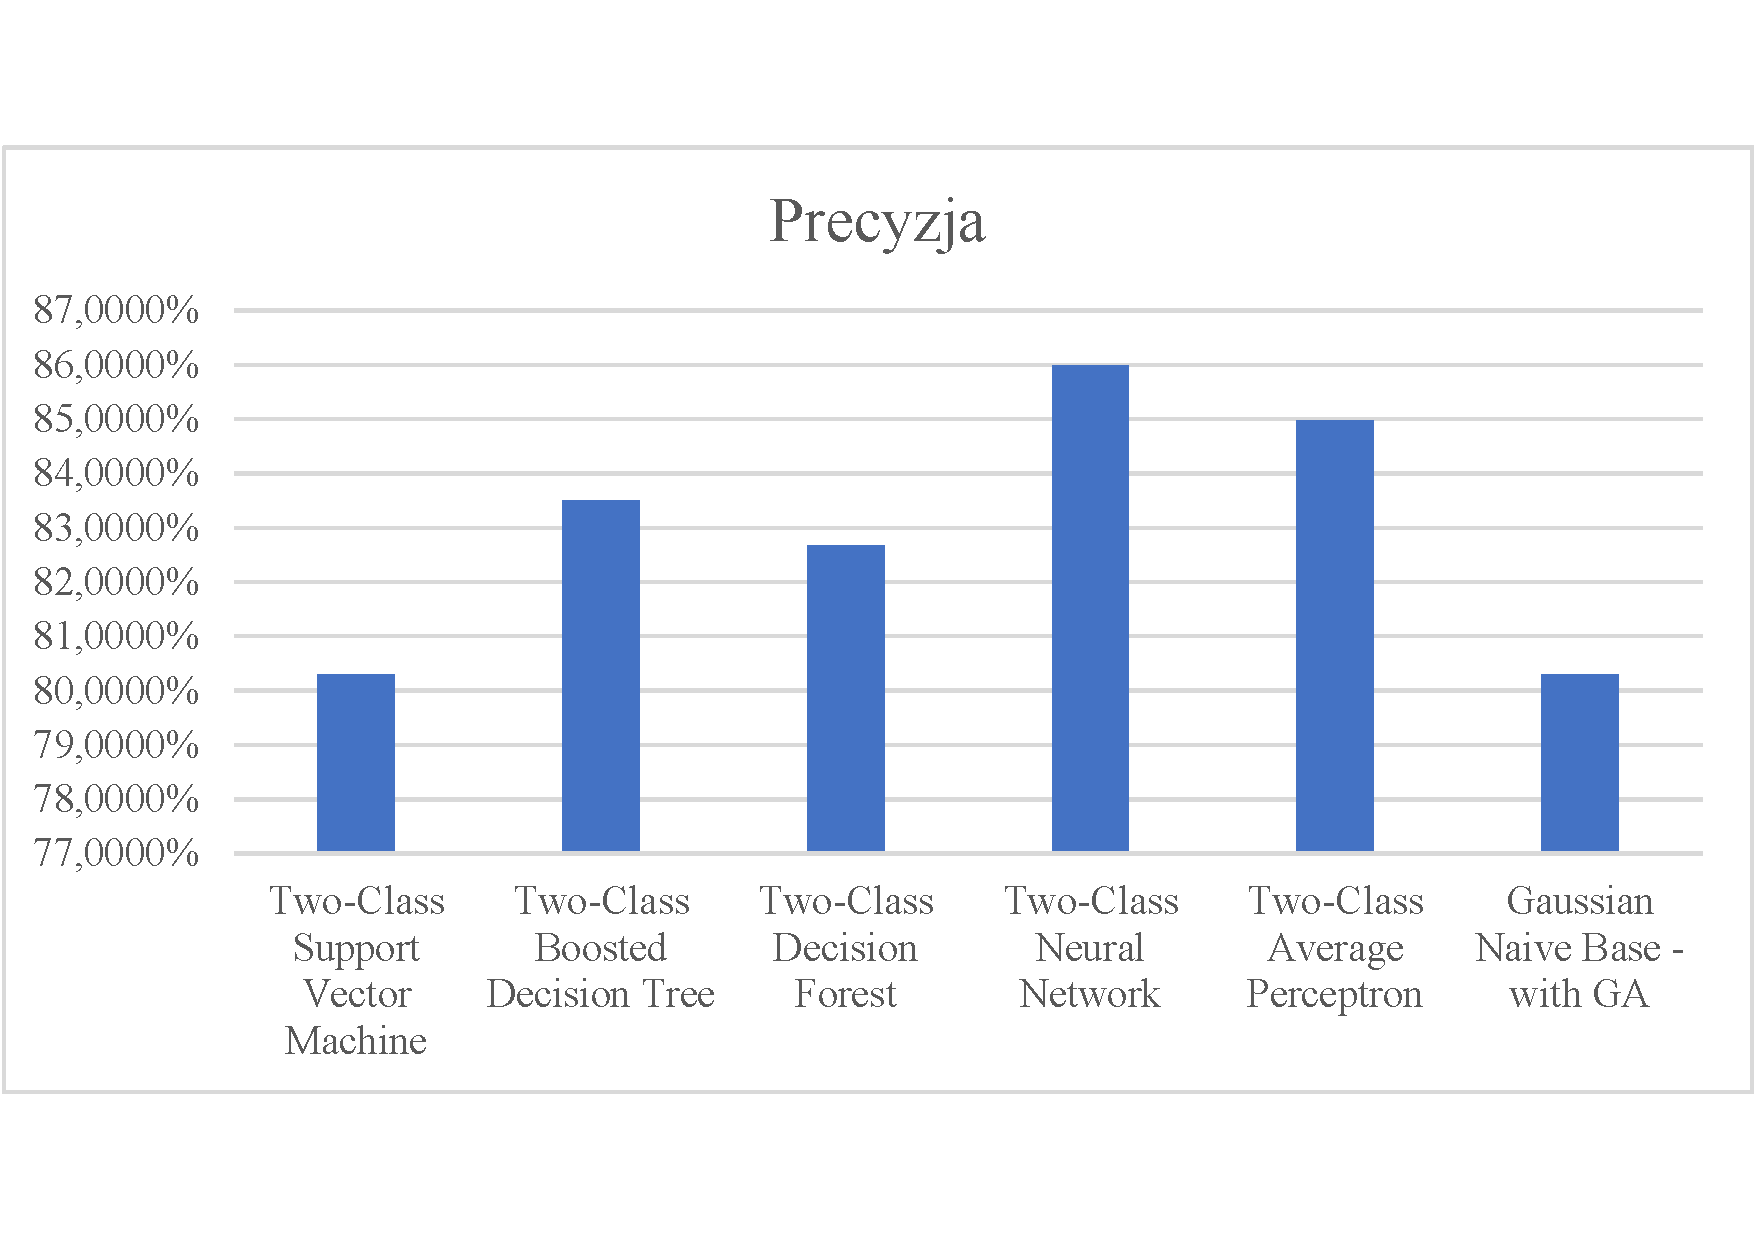
\includegraphics[width=\textwidth]{images/prec-res}
    \captionsource{Precyzja algorytmów}{Opracowanie własne}
    \label{fig:acc-prec}
\end{figure}

\subsection{Czułośc}
Wszystkie wpisy klasy ''\textbf{1}'' zostały poprawnie sklasyfikowane przez algorytm ''\textit{Gaussian Naive Base - with GA}'' ($100\%$), najsłabiej poradził sobie ''\textit{Two-Class Neural Network}'' ($96,7705\%$). Wartości zostały przedstawione w \refsource{tabeli}{tab:rec-res} oraz na \refsource{wykresie}{fig:rec-res}.

\begin{table}[H]
    \centering
    \captionsource{Wynik czułości algorytmów}{Opracowanie własne}
    \begin{tabular}{|l|r|} \hline
    \textbf{Algorytm} & \textbf{Wartość} \\ \hline
    Two-Class Support Vector Machine & $99,9998\%$ \\ \hline
    Two-Class Boosted Decision Tree & $99,5563\%$ \\ \hline
    Two-Class Decision Forest & $99,9996\%$ \\ \hline
    Two-Class Neural Network & $96,7705\%$ \\ \hline
    Two-Class Average Perceptron & $99,9531\%$ \\ \hline
    Gaussian Naive Base - with GA & $100\%$ \\ \hline
    \end{tabular}
    \label{tab:acc-rec}
\end{table}

\begin{figure}[H]
    \centering
    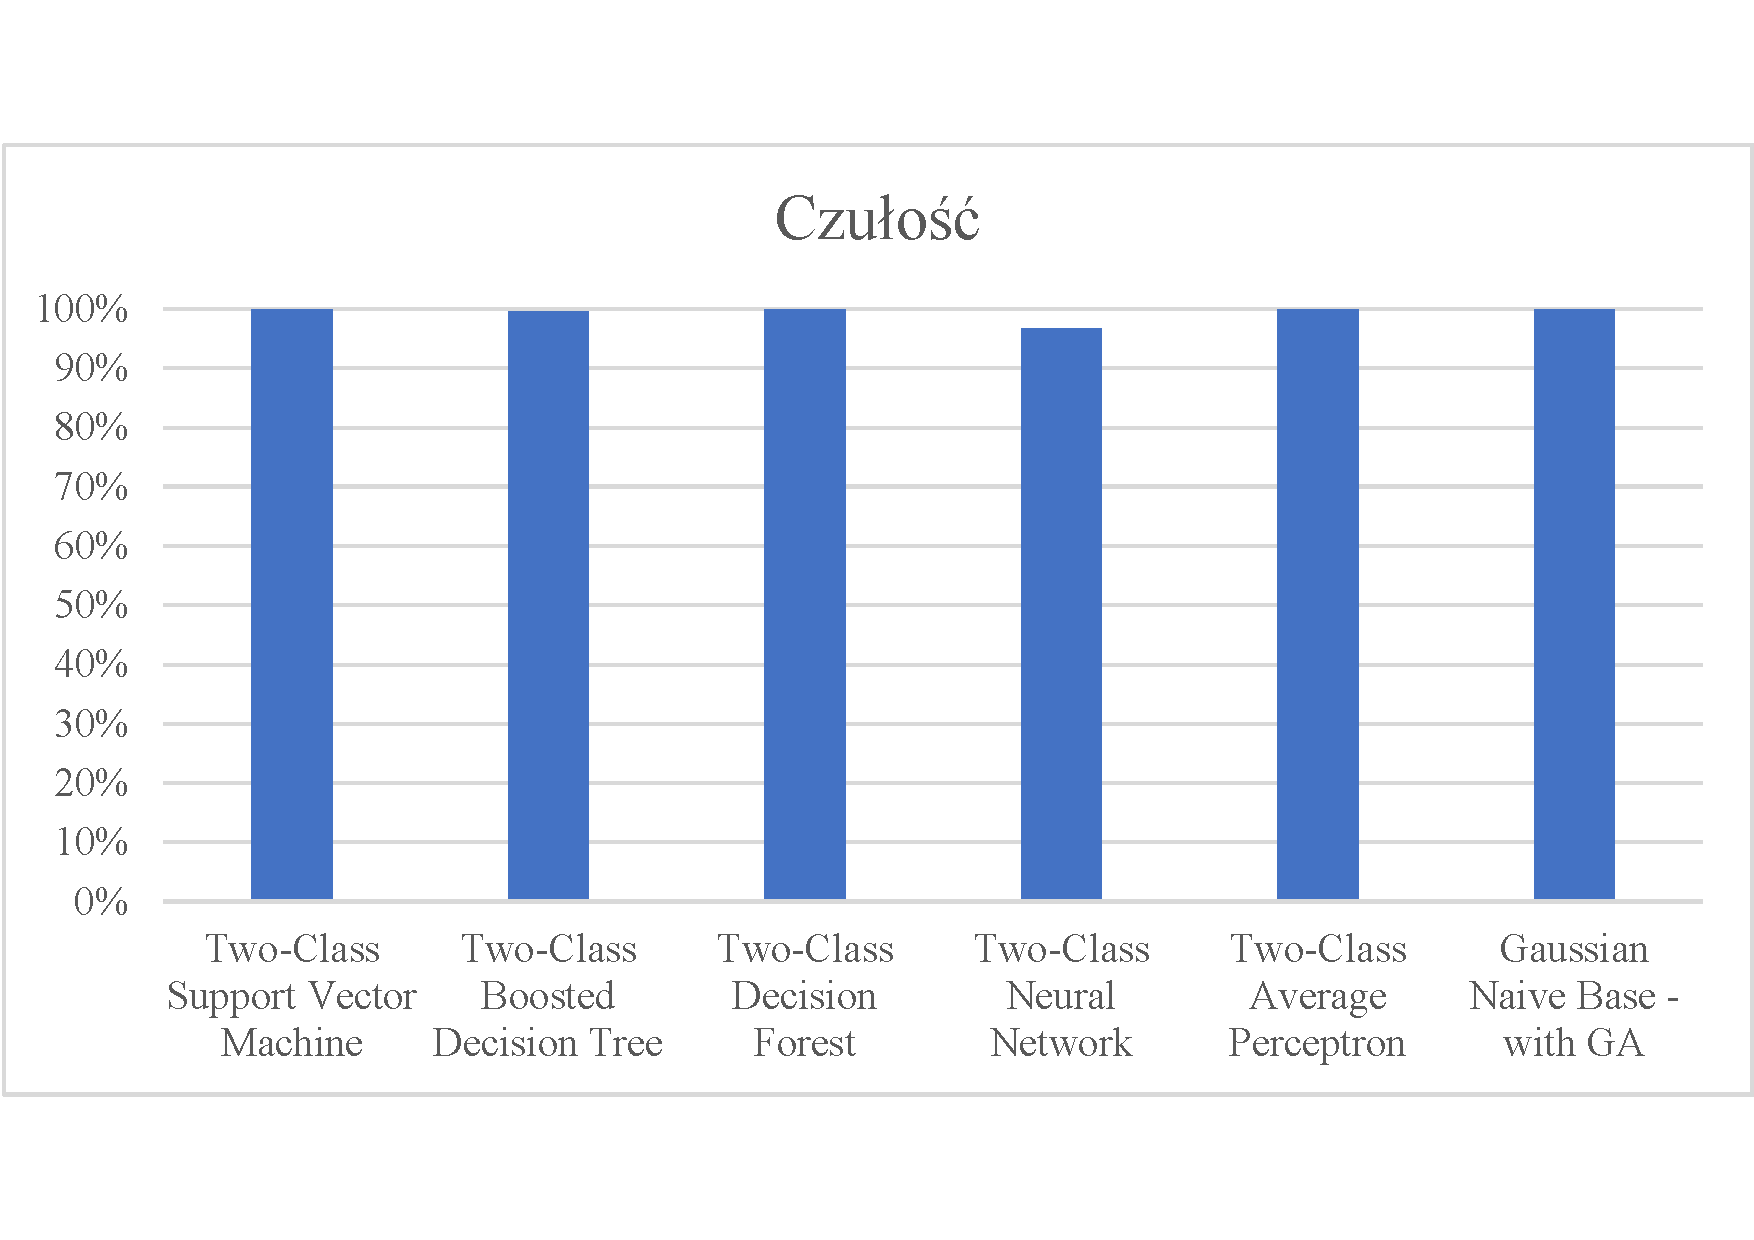
\includegraphics[width=\textwidth]{images/rec-res}
    \captionsource{Czułość algorytmów}{Opracowanie własne}
    \label{fig:rec-res}
\end{figure}

\subsection{F1}
Największą wartość F1 uzyskał ''\textit{Two-Class Average Perceptron}'' ($91,8608\%$). Najmniejszą uzyskał ''\textit{Two-Class Support Vector Machine}'' ($89,0739\%$). GAGNB w tym teście uzyskał $89,0740\%$. Wyniki zostały przedstawione w \refsource{tabeli}{tab:acc-f1} oraz na \refsource{wykresie}{fig:f1-res}.

\begin{table}[H]
    \centering
    \captionsource{Wynik F1 algorytmów}{Opracowanie własne}
    \begin{tabular}{|l|r|} \hline
    \textbf{Algorytm} & \textbf{Wartość} \\ \hline
    Two-Class Support Vector Machine & $89,0739\%$ \\ \hline
    Two-Class Boosted Decision Tree & $90,8249\%$ \\ \hline
    Two-Class Decision Forest & $90,5159\%$ \\ \hline
    Two-Class Neural Network & $91,0553\%$ \\ \hline
    Two-Class Average Perceptron & $91,8608\%$ \\ \hline
    Gaussian Naive Base - with GA & $89,0740\%$ \\ \hline
    \end{tabular}
    \label{tab:acc-f1}
\end{table}

\begin{figure}[H]
    \centering
    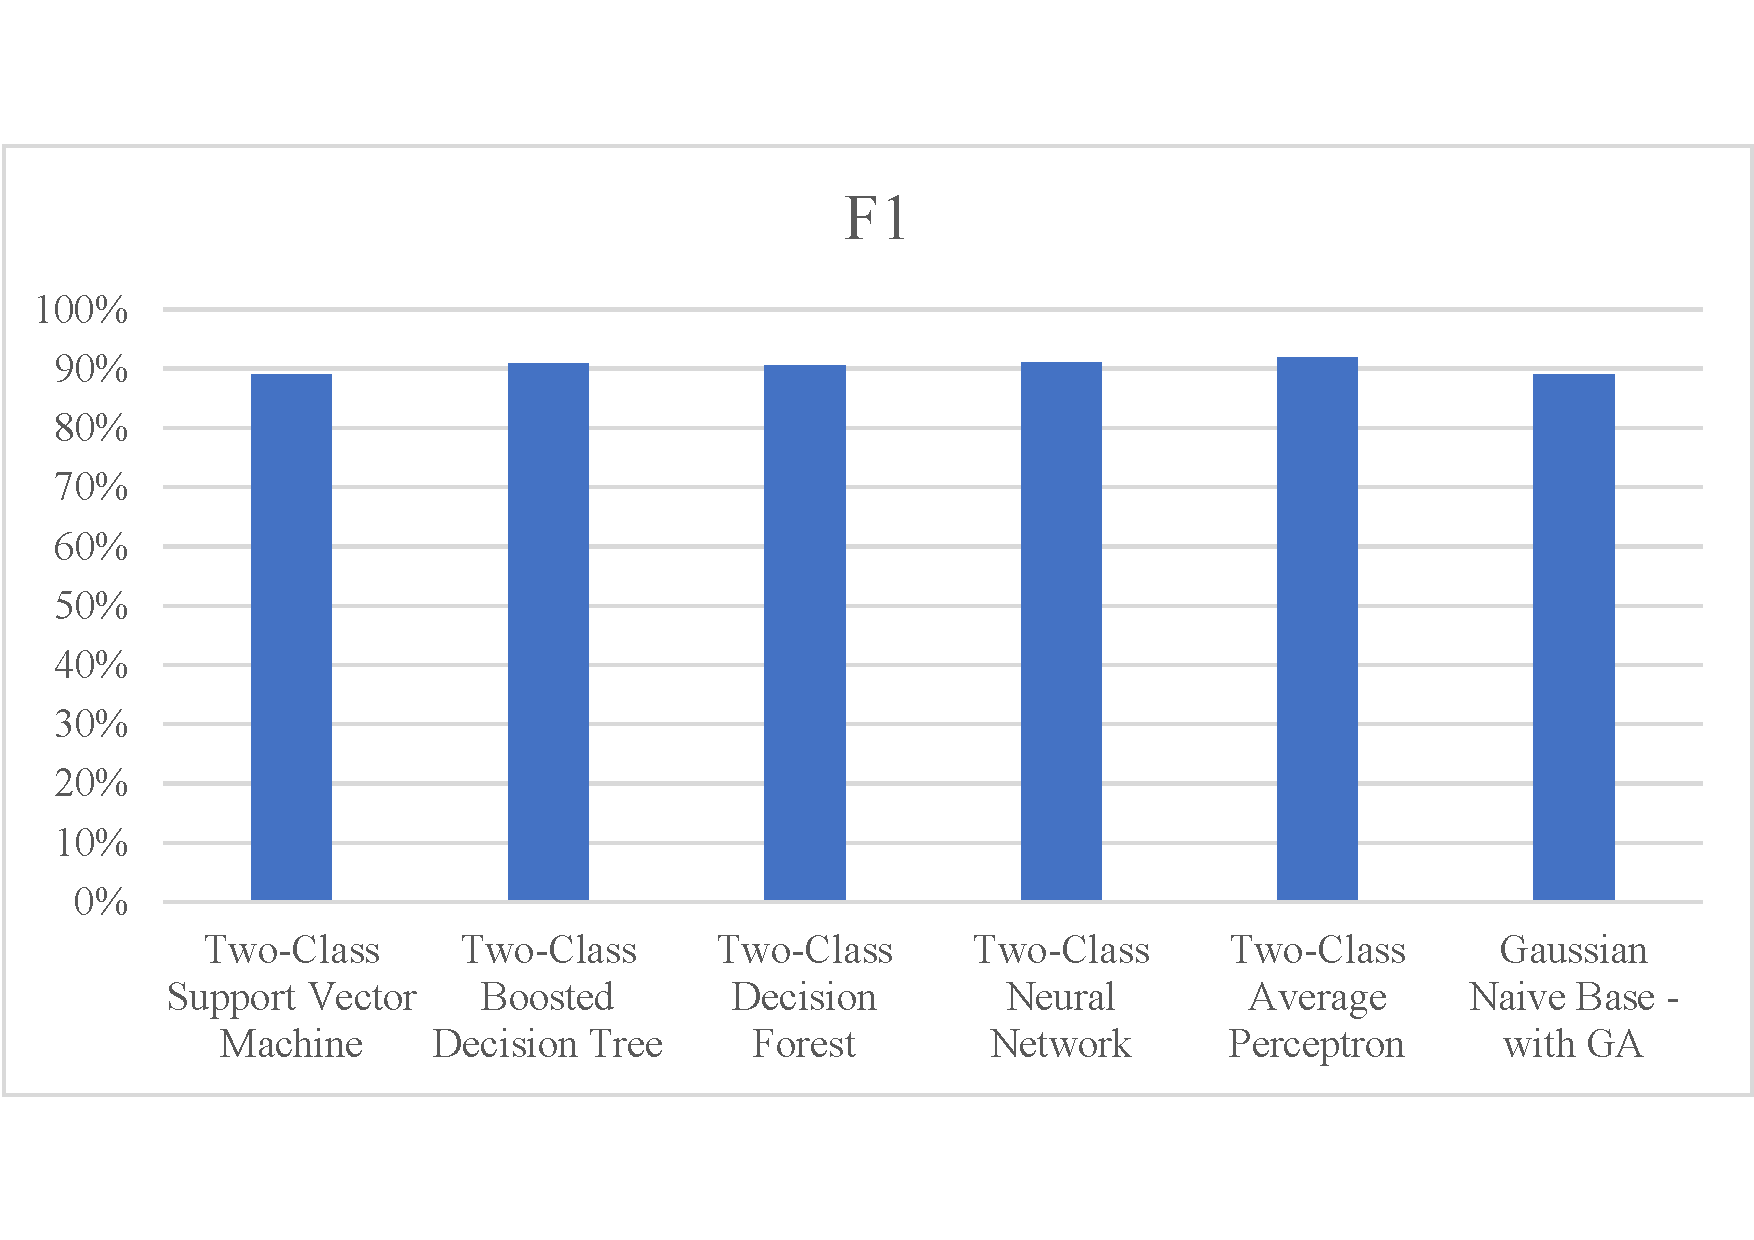
\includegraphics[width=\textwidth]{images/f1-res}
    \captionsource{F1 algorytmów}{Opracowanie własne}
    \label{fig:f1-res}
\end{figure}

\subsection{AUC}
Analizując wynik AUC, można zauważyć, że najlepsza sprawność również uzyskał algorytm ''\textit{Two-Class Average Perceptron}'' ($79,1292\%$). Najgorszy algorytm to znów algorytm wykorzystujący SVM ($49,9999\%$), wynik wskazał na to, że algorytm ten miał niższą sprawność niż próba losowa. W tym teście sprawność algorytmu GAGNB wyniosła $50\%$. Wyniki przedstawiono w \refsource{tabeli}{tab:acc-auc} oraz na \refsource{wykresie}{fig:auc-res}.

\begin{table}[H]
    \centering
    \captionsource{Wynik czułości algorytmów}{Opracowanie własne}
    \begin{tabular}{|l|r|} \hline
    \textbf{Algorytm} & \textbf{Wartość} \\ \hline
    Two-Class Support Vector Machine & $49,9999\%$ \\ \hline
    Two-Class Boosted Decision Tree & $69,9089\%$ \\ \hline
    Two-Class Decision Forest & $63,5244\%$ \\ \hline
    Two-Class Neural Network & $72,1864\%$ \\ \hline
    Two-Class Average Perceptron & $79,1892\%$ \\ \hline
    Gaussian Naive Base - with GA & $50\%$ \\ \hline
    \end{tabular}
    \label{tab:acc-auc}
\end{table}

\begin{figure}[H]
    \centering
    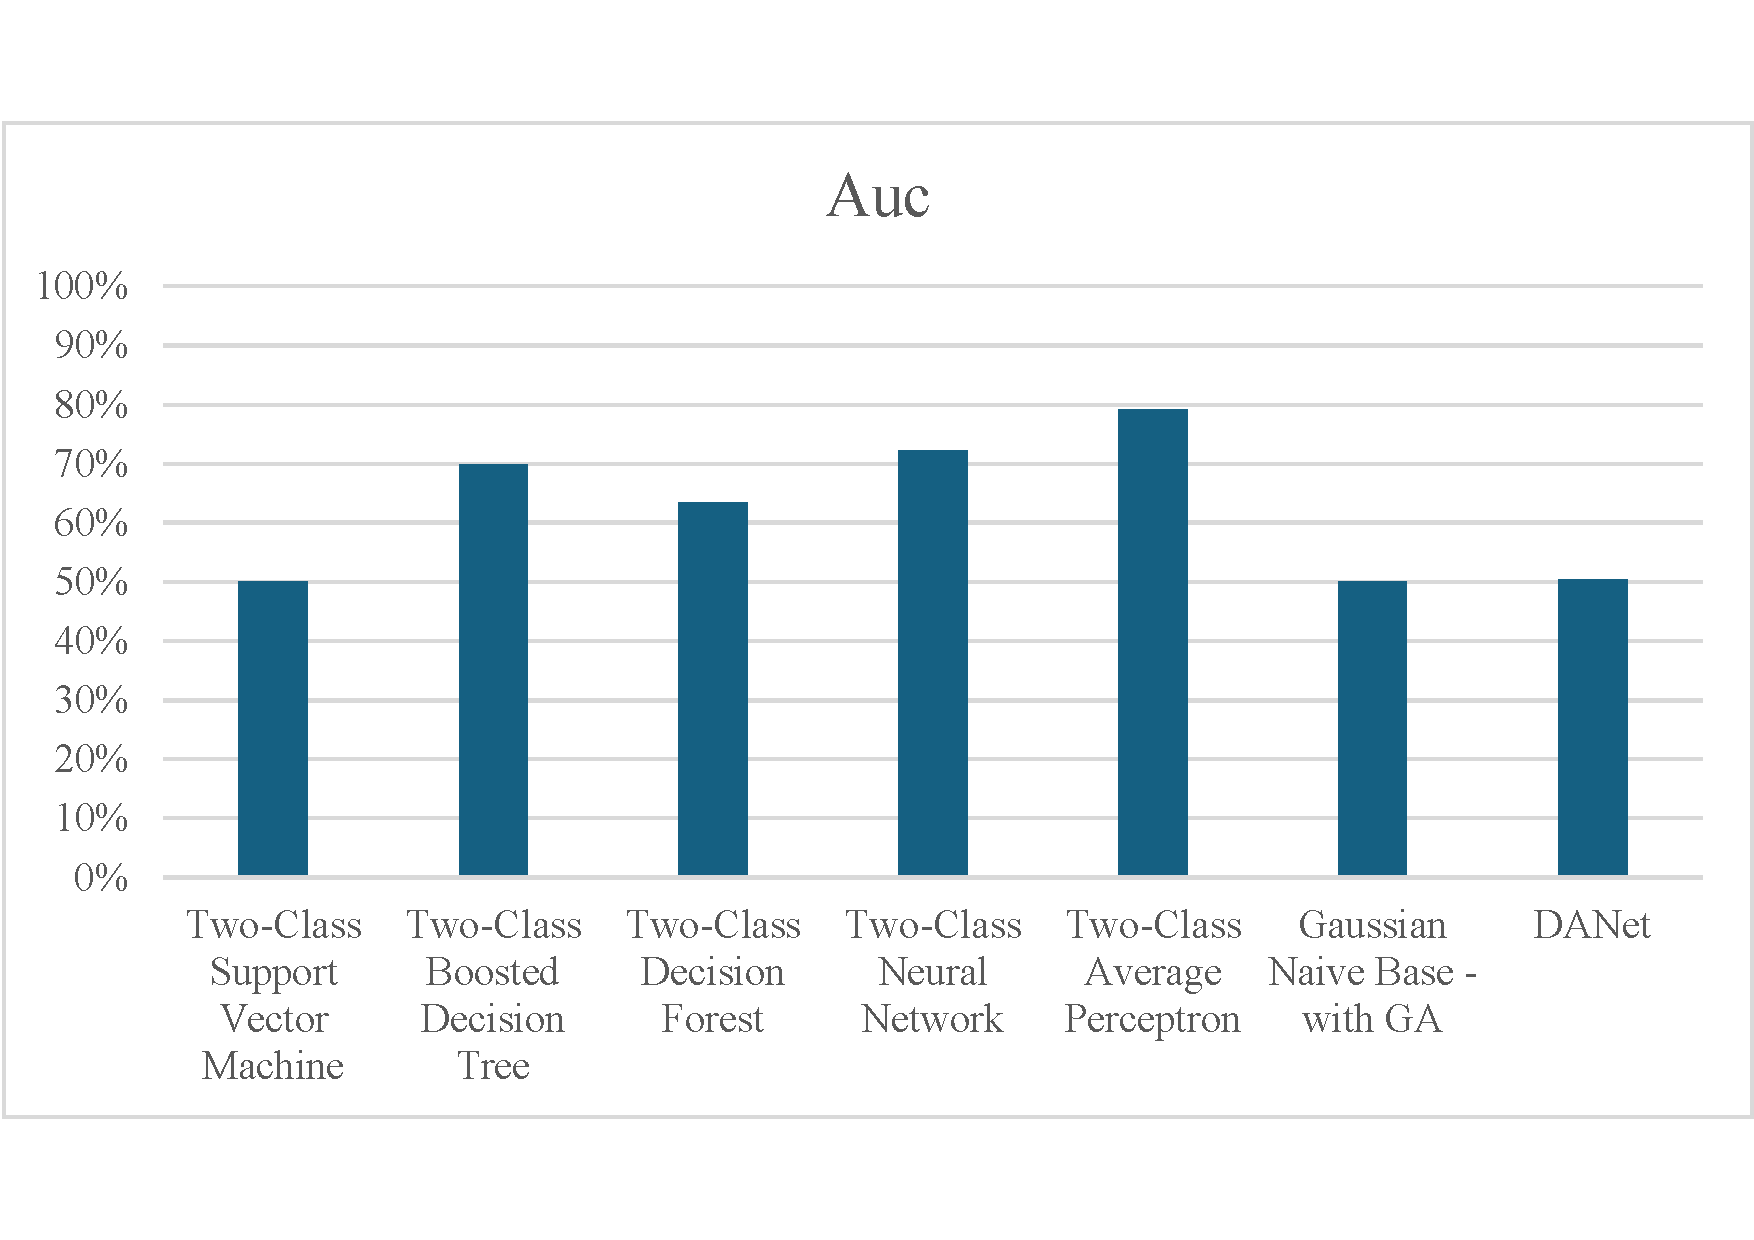
\includegraphics[width=\textwidth]{images/auc-res}
    \captionsource{AUC algorytmów}{Opracowanie własne}
    \label{fig:auc-res}
\end{figure}

\section{Wnioski}

